\documentclass[10pt,a4paper]{article}
\usepackage[utf8]{inputenc}
\usepackage[english]{babel}
\usepackage[T1]{fontenc}
\usepackage{amsmath}
\usepackage{amsfonts}
\usepackage{amssymb}
\usepackage{makeidx}
\usepackage{graphicx}
\usepackage{fourier}
\usepackage{listings}
\usepackage{color}
\usepackage{hyperref}
\usepackage[left=2cm,right=2cm,top=2cm,bottom=2cm]{geometry}
\author{Johannes Scheller, Vincent Noculak, Lukas Powalla, Richard Asbah}
\title{Computational Physics - Project 4}

\lstset{language=C++,
	keywordstyle=\bfseries\color{blue},
	commentstyle=\itshape\color{red},
	stringstyle=\color{green},
	identifierstyle=\bfseries,
	frame=single}
\begin{document}

\maketitle
\newpage
\tableofcontents
\newpage


\section{Results}

%	e part:

In figure \ref{e_all}, \ref{absm_all}, \ref{chi_all} and \ref{cv_all}, the expectation values $<E>$ and $<|M|>$, the specific heat $C_V$ and the susceptibility $\chi$ for lattice sizes $L = 20, 40, 60, 80$ can be seen as functions of $T$ close to the critical temperature. It is the easiest to estimate the critical temperature by looking at figure \ref{cv_all}, because it is at the temperature where $C_V$ is the highest. In figure \ref{cv2040} and \ref{cv6080} we increased the number of Monte Carlo cycles and decreased the temperature step length and interval to determine the temperature of the maximum of $C_V$ more precisely. In table \ref{tc} the measured critical temperatures can be seen. While it is possible to measure $T_C$ even more precisely by increasing the Monte Carlo cycles and decreasing the Temperature step length, it is not possible aim at any precision, due to the quickly increasing calculation time.


\begin{figure}[h]
	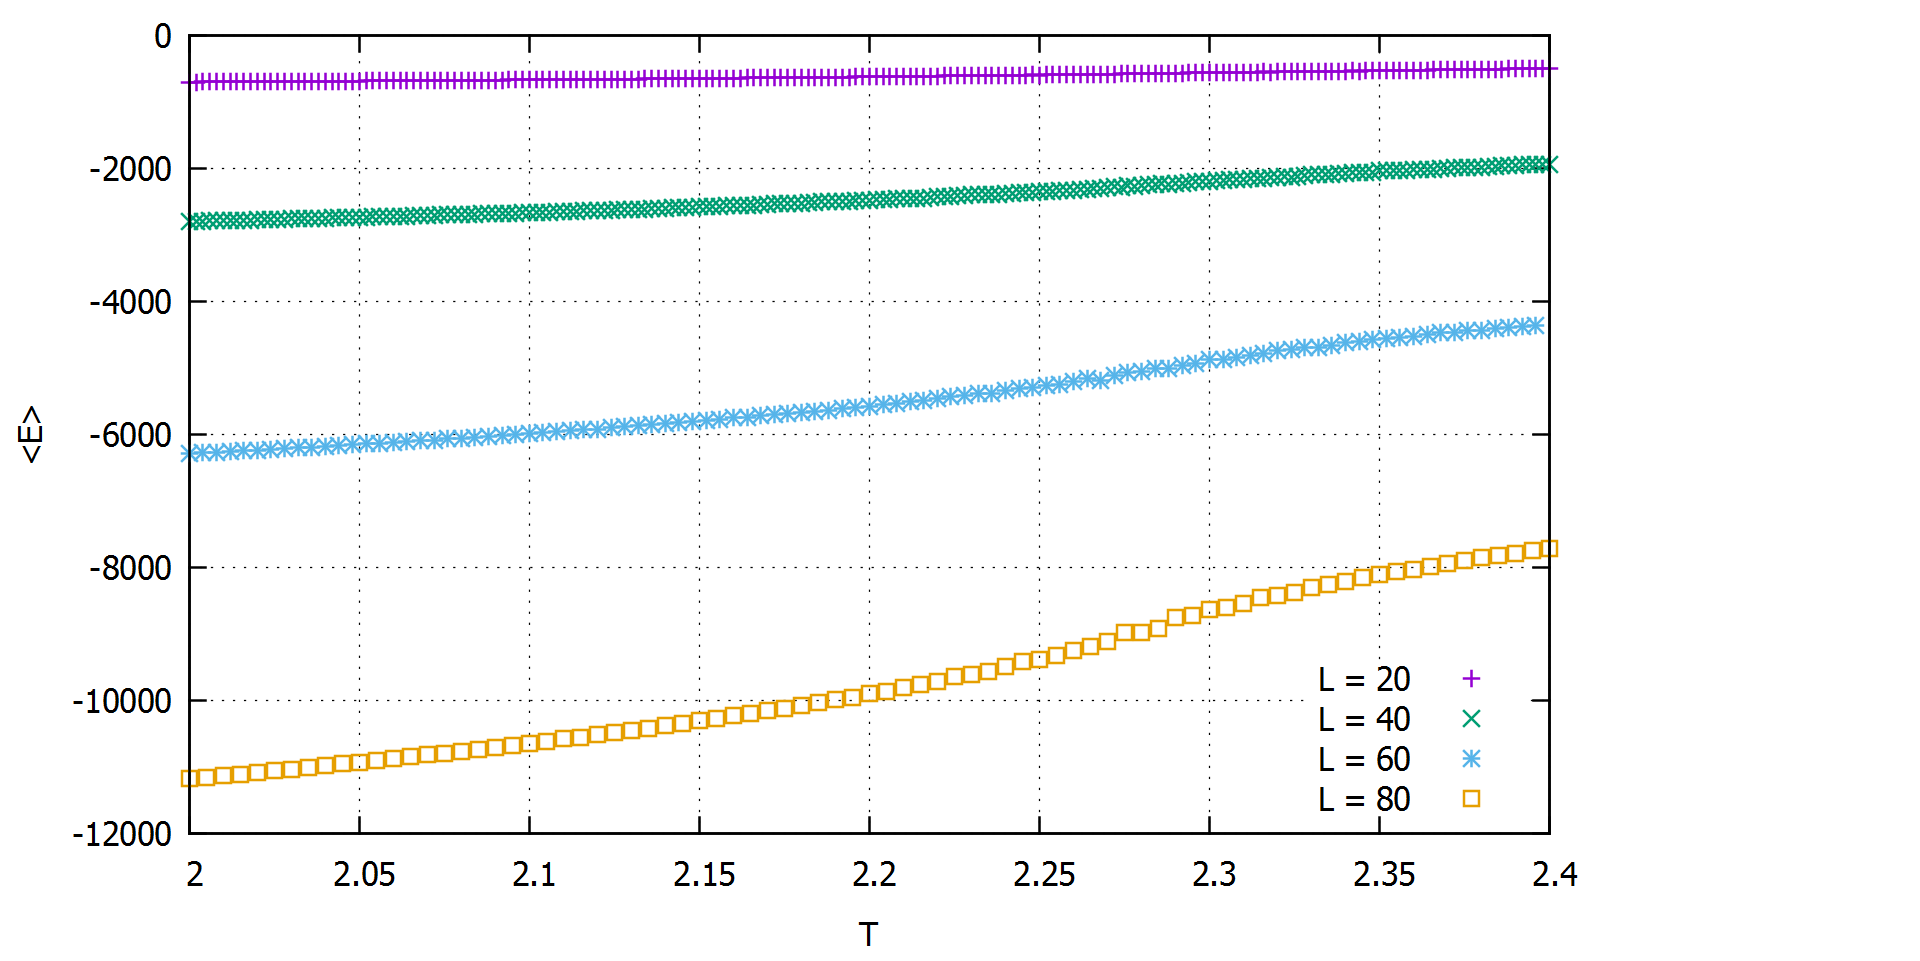
\includegraphics[scale = 0.25]{E_all.png}
	\centering
	\caption{Expectation value of the energy against temperature for different lattice sizes ($10^6$ Monte Carlo cycles)}
	\label{e_all}
\end{figure}

\begin{figure}[h]
	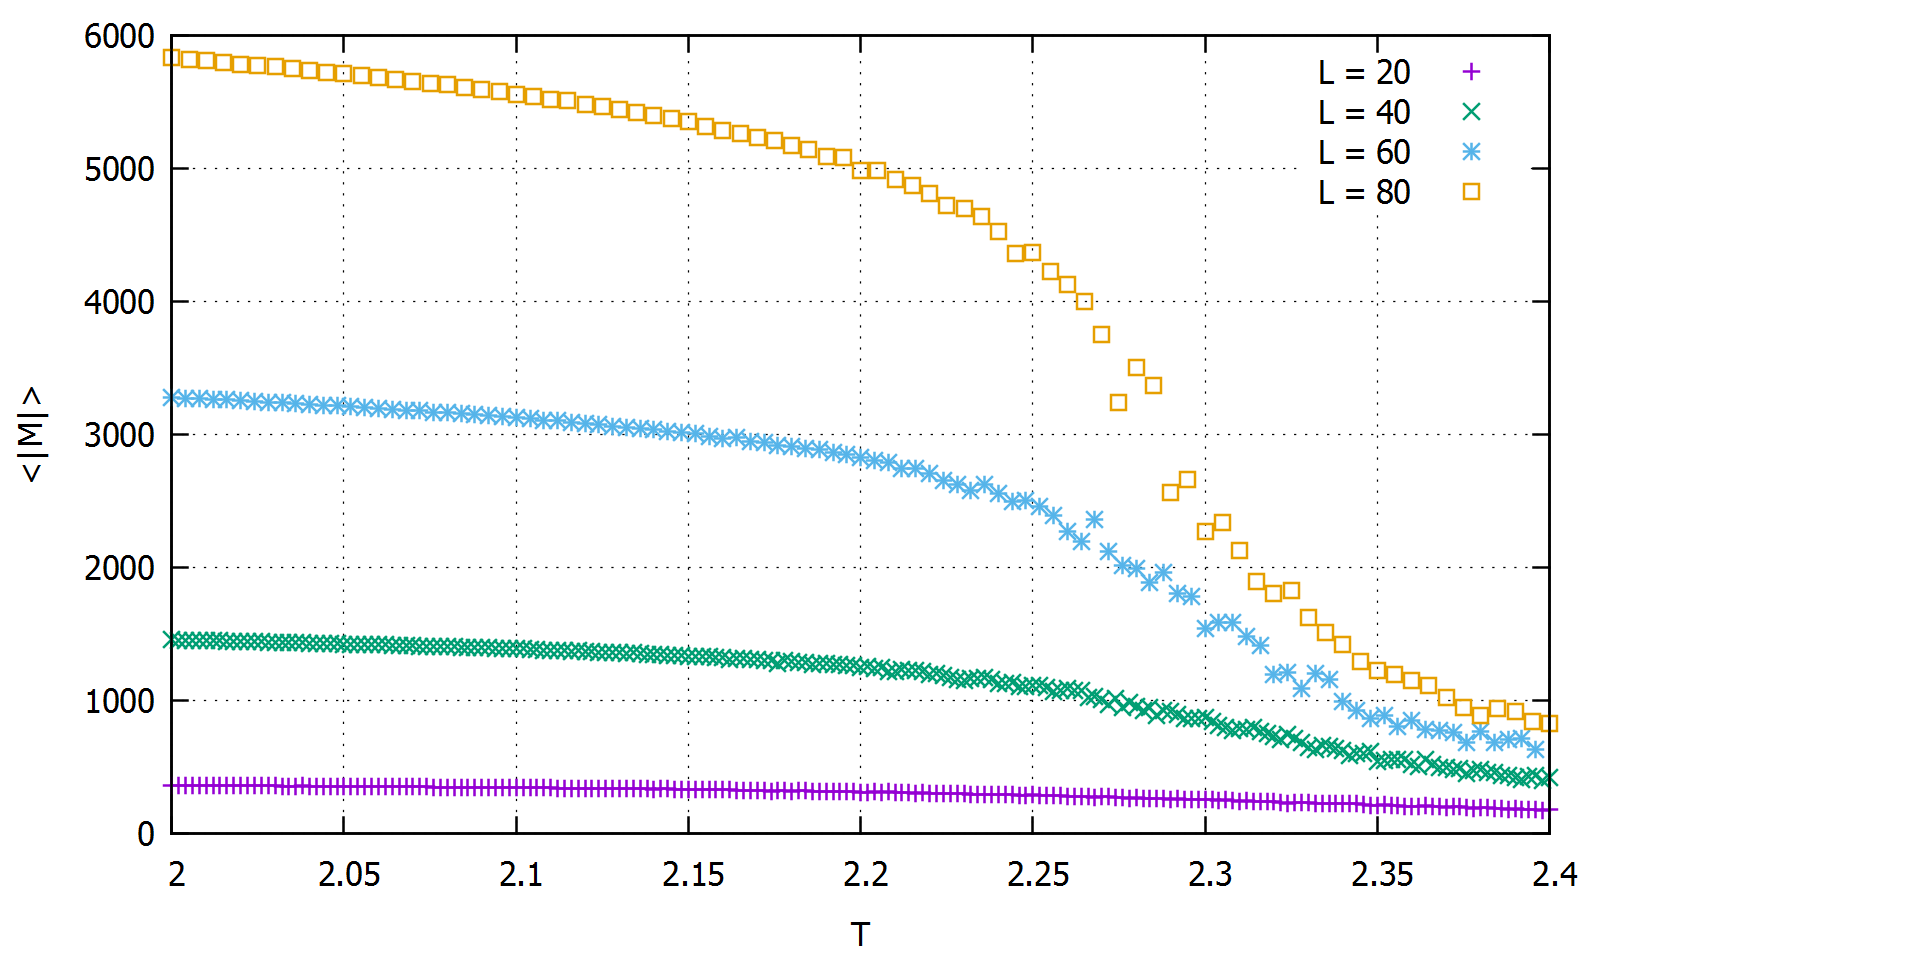
\includegraphics[scale = 0.25]{absm_all.png}
	\centering
	\caption{Expectation value of the absolute magnetisation against temperature for different lattice sizes ($10^6$ Monte Carlo cycles)}
	\label{absm_all}
\end{figure}

\begin{figure}[h]
	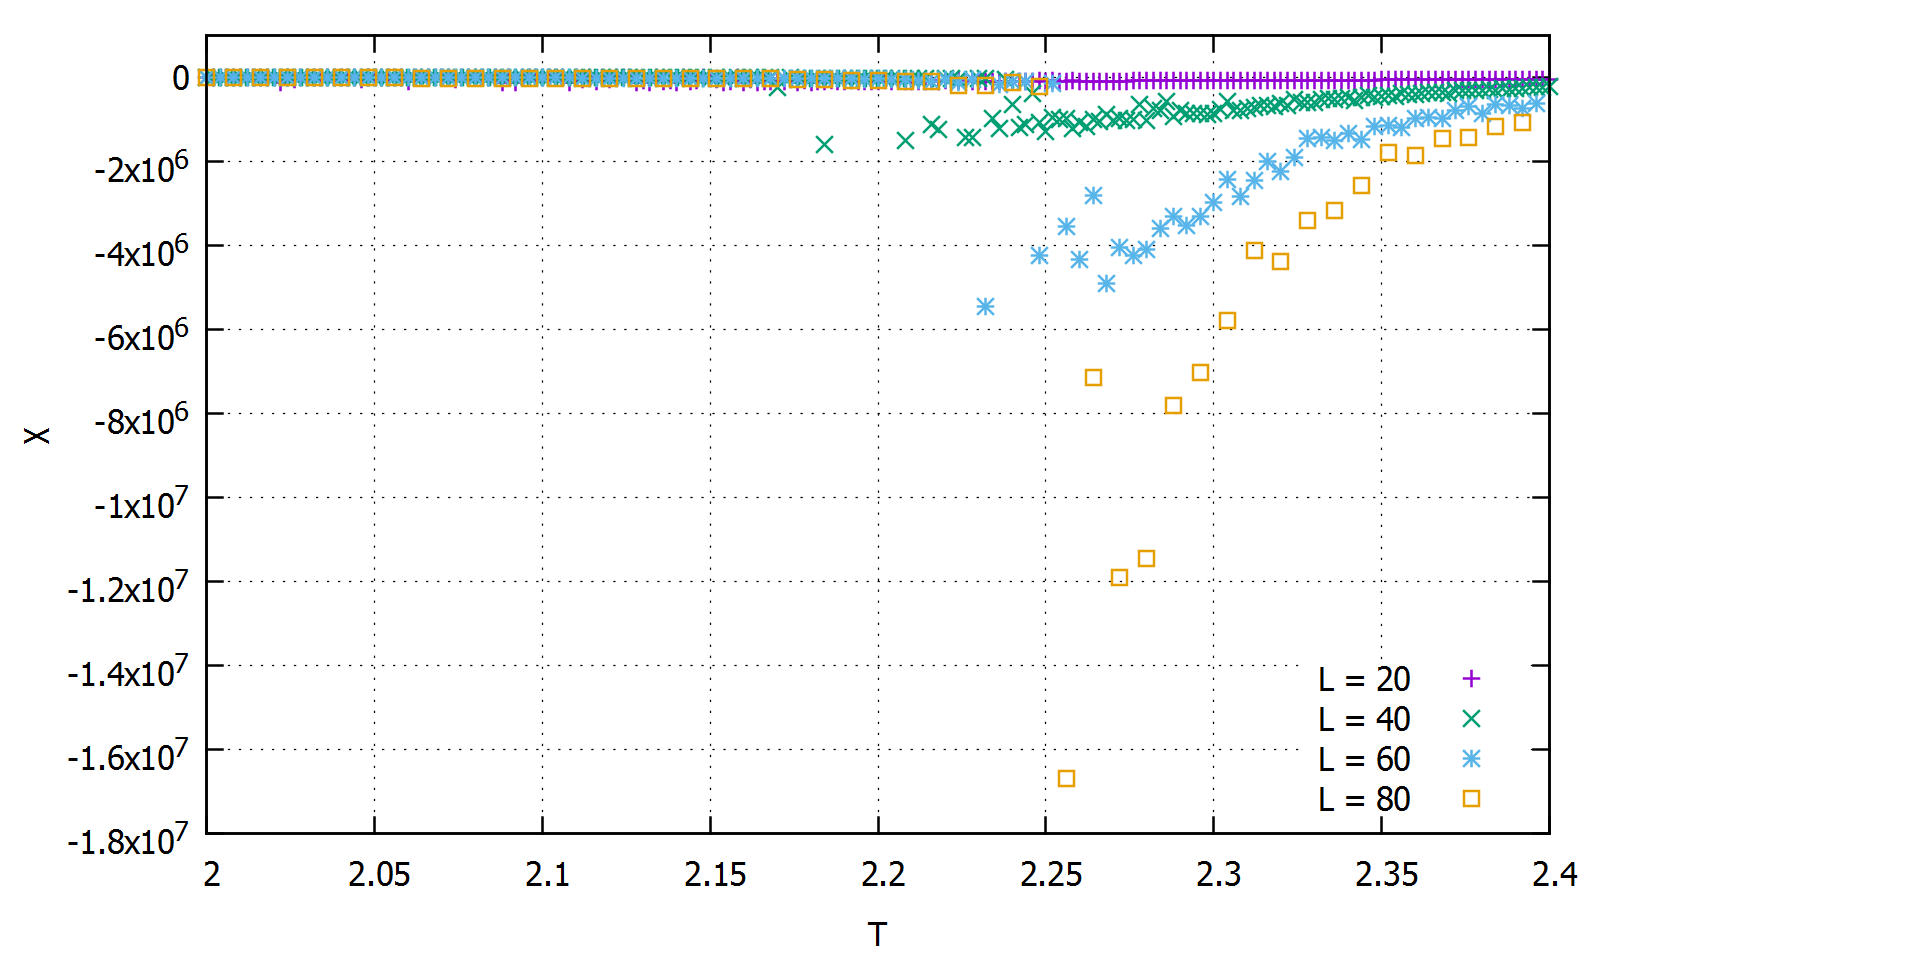
\includegraphics[scale = 0.25]{sus_all.png}
	\centering
	\caption{Susceptibility against temperature for different lattice sizes ($10^6$ Monte Carlo cycles)}
	\label{chi_all}
\end{figure}

\begin{figure}[h]
	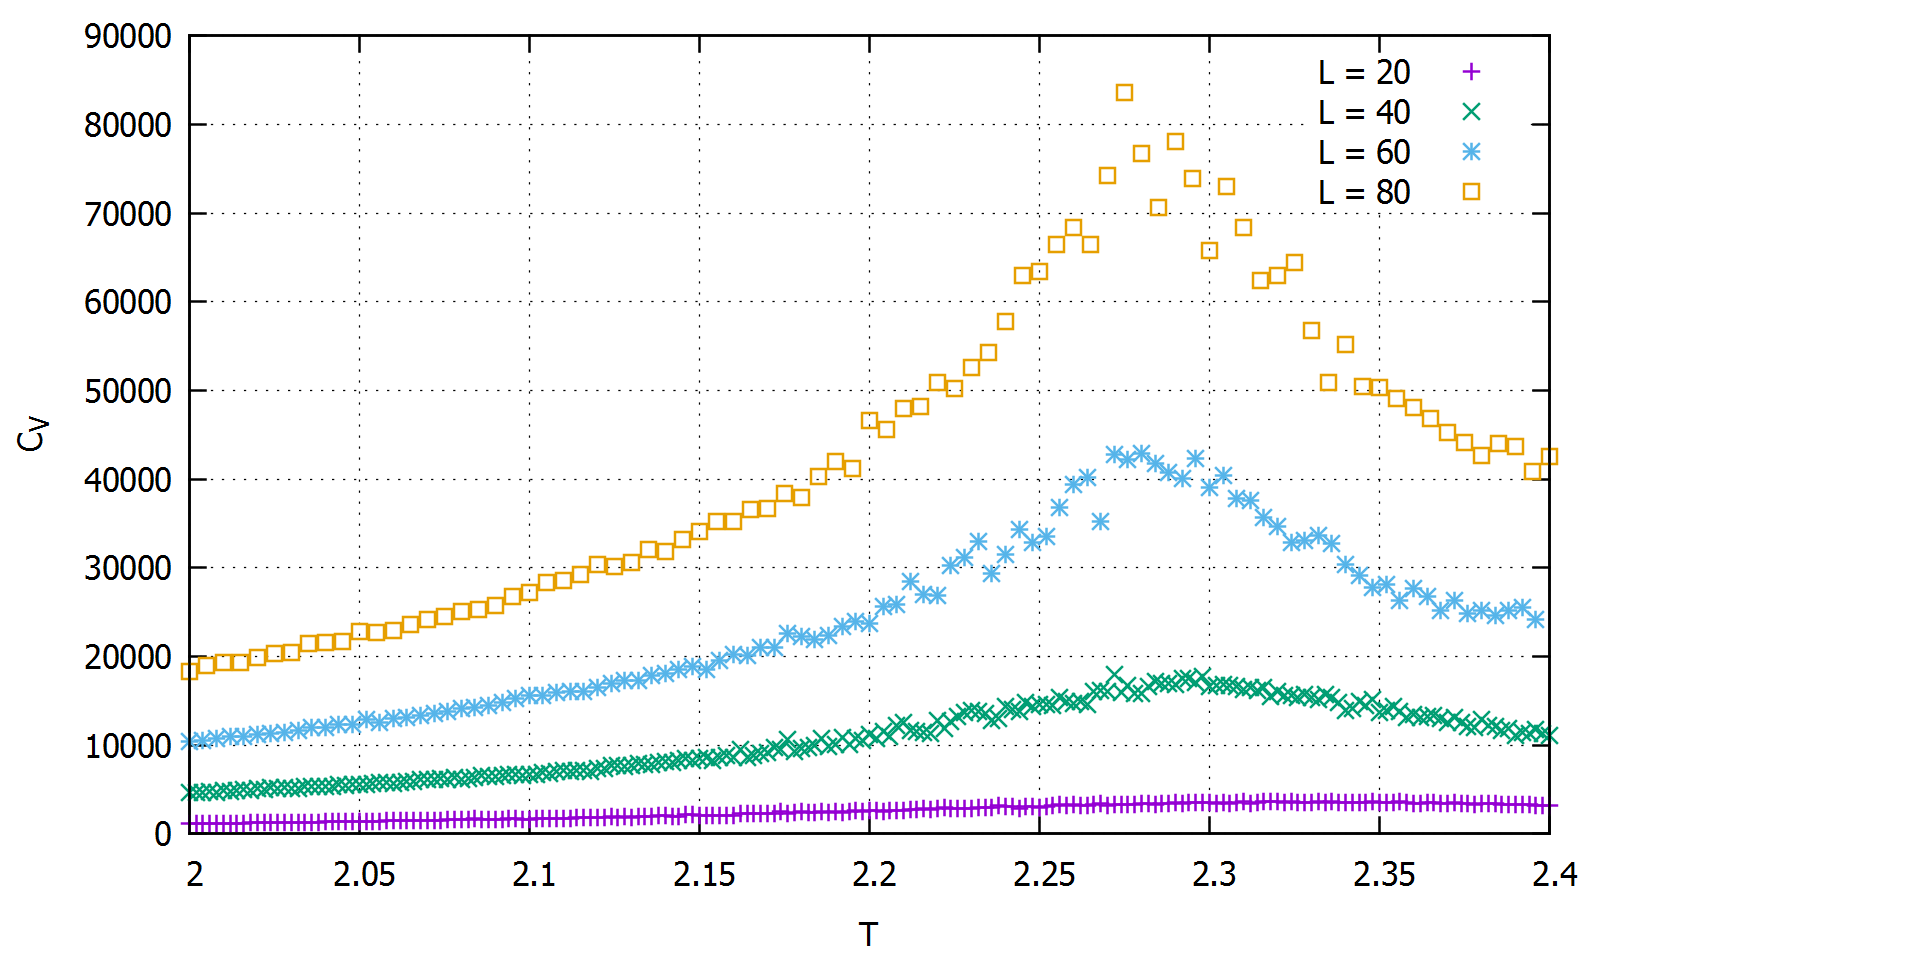
\includegraphics[scale = 0.25]{cv_all.png}
	\centering
	\caption{Expectation value of the specific heat against temperature for different lattice sizes ($10^6$ Monte Carlo cycles)}
	\label{cv_all}
\end{figure}

\begin{figure}[h]
	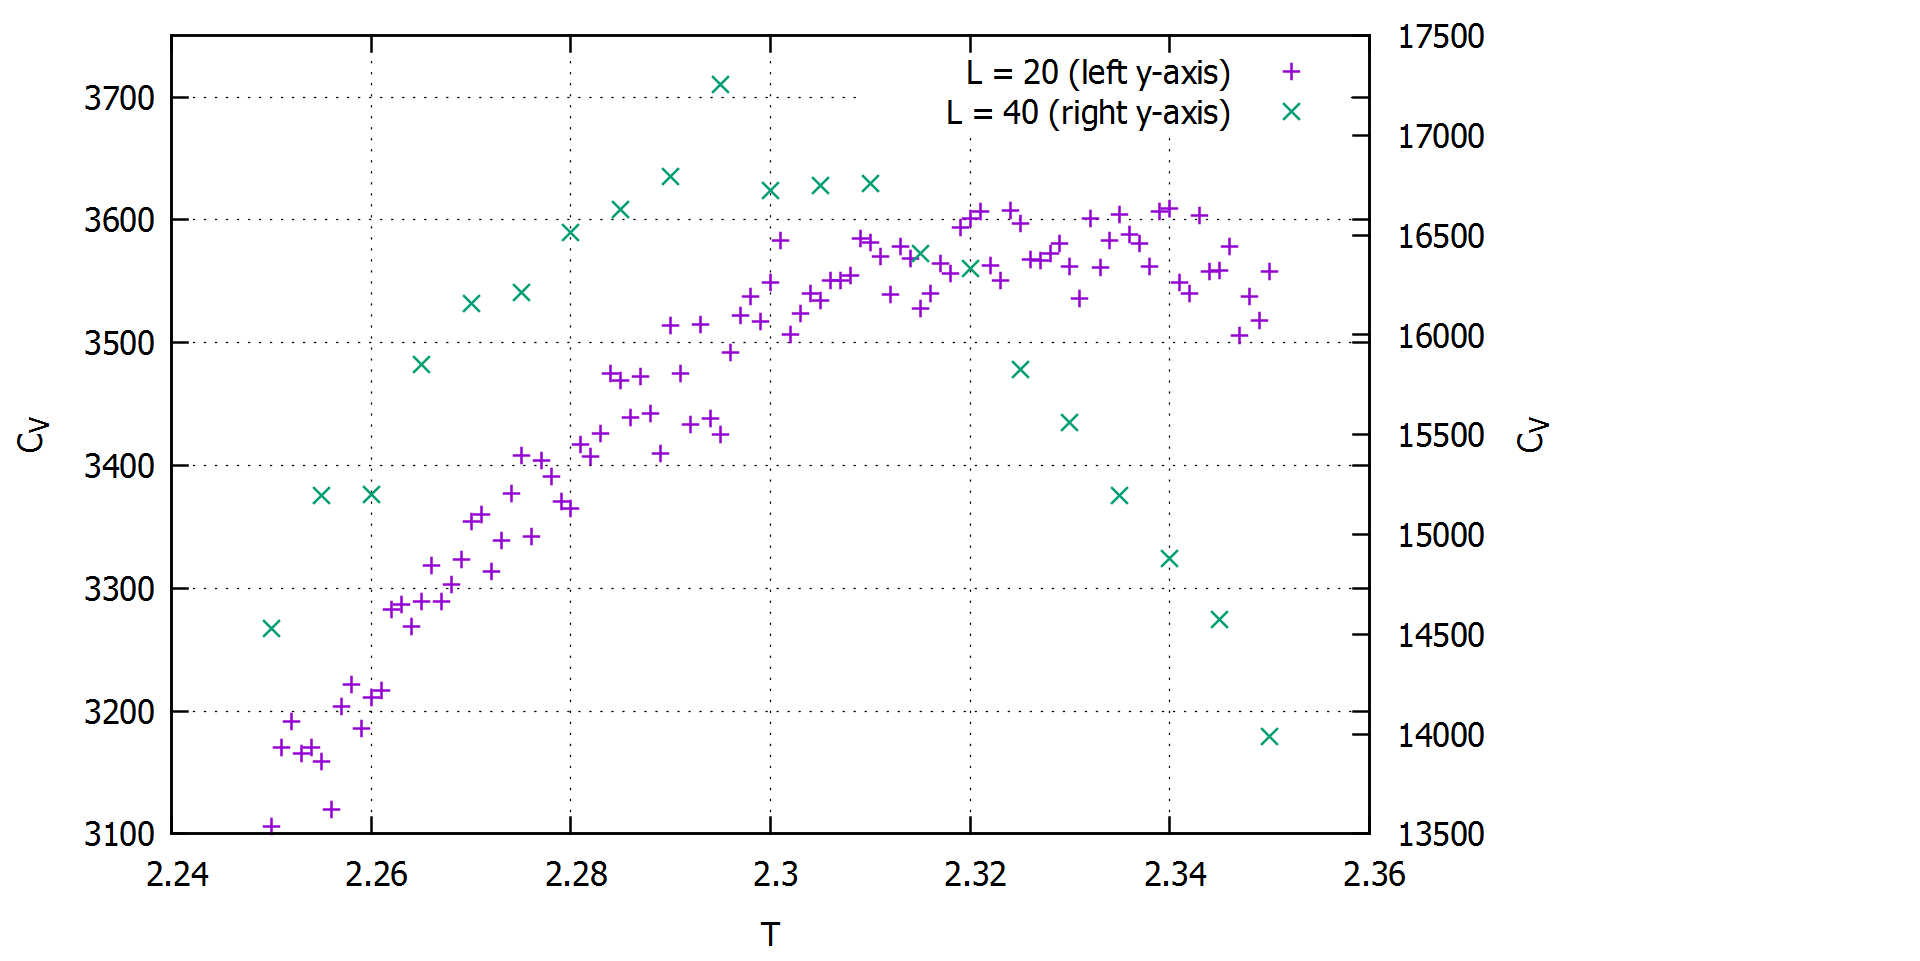
\includegraphics[scale = 0.25]{cv2040.png}
	\centering
	\caption{Expectation value of the specific heat against temperature for lattice sizes L = 20 and L = 40 ($5 \cdot 10^6$ Monte Carlo cycles)}
	\label{cv2040}
\end{figure}

\begin{figure}[h]
	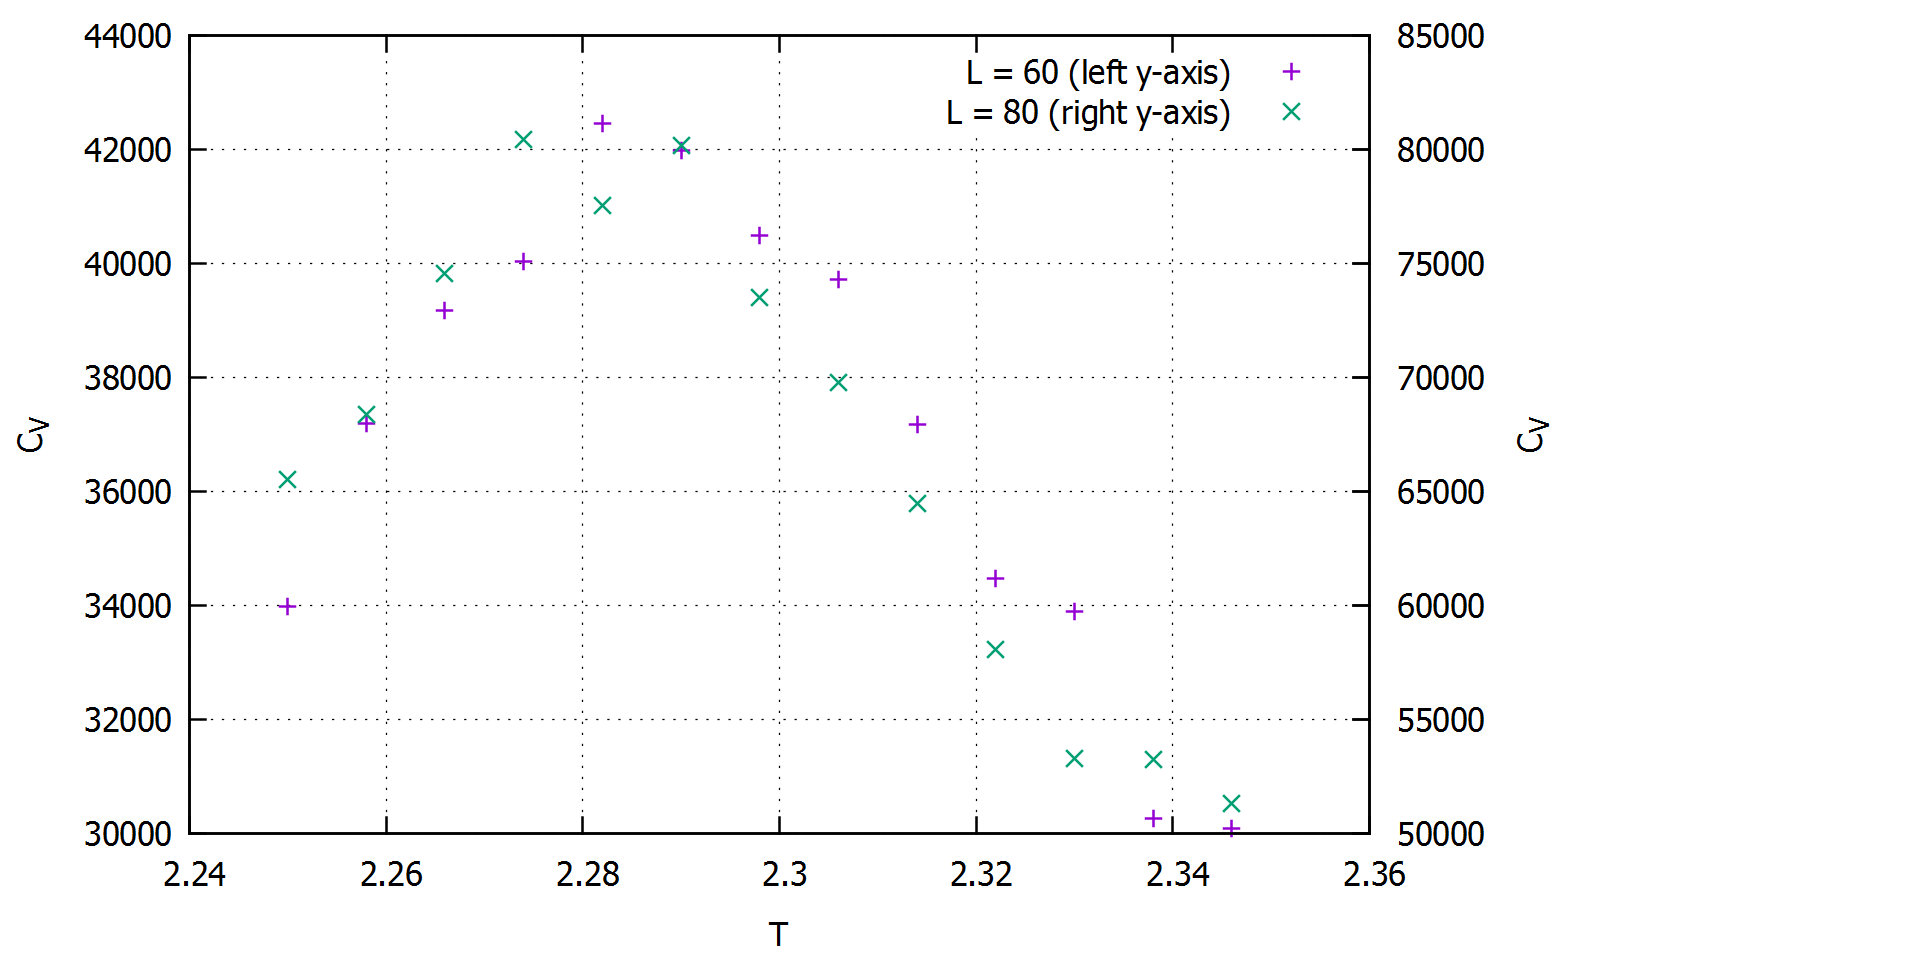
\includegraphics[scale = 0.25]{cv6080.png}
	\centering
	\caption{Expectation value of the specific heat against temperature for lattice sizes L = 60 and L = 80 ($5 \cdot 10^6$ Monte Carlo cycles)}
	\label{cv6080}
\end{figure}

\begin{table}[h!]
	\centering
	\begin{tabular}{|l|r|c|lrp{16cm}}\hline
		L & $T_C$ \\\hline
		20 & $(2.33 \pm 0.01)$\\
		40 & $(2.295 \pm 0.007)$\\
		60 & $(2.285 \pm 0.005)$\\
		80 & $(2.280 \pm 0.007)$\\\hline
	\end{tabular}
	\caption{Critical temperature for different lattice sizes L }
	\label{tc}
\end{table}

\begin{figure}[h]
	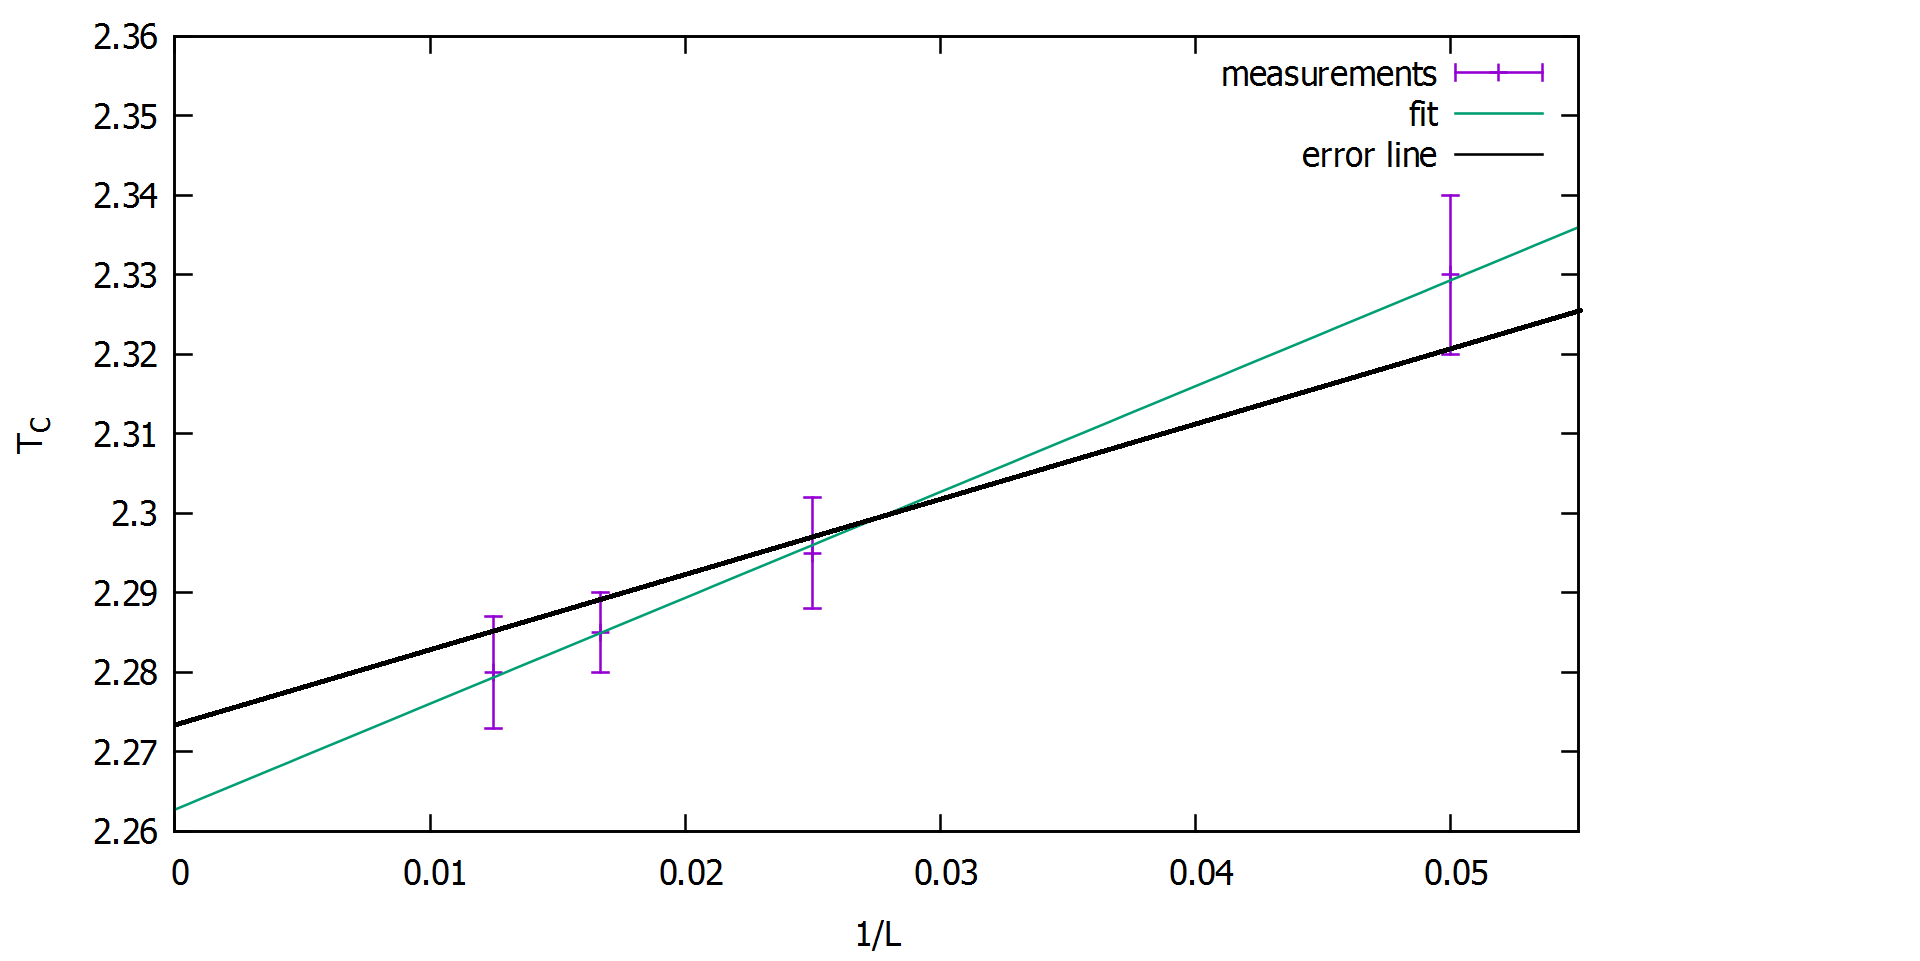
\includegraphics[scale = 0.25]{tc2.png}
	\centering
	\caption{Critical temperature $T_C$ against $\frac{1}{L}$}
	\label{tc2}
\end{figure}









\end{document}